\chapter{Introducción al aprendizaje por refuerzo}

\lecture{3}{2020-06-12}{Introducción a tensorflow}

Está todo en Jupyter.

\lecture{4}{2020-06-12}{Introducción a RL}

\section{Procesos de decisión de Markov (MDP)}%
\label{sec:procesos_de_decisión_de_markov_mdp_}

Los MDP quedan definidos por: $s, a, r(s, a) \textrm{ y } p(s'|s,a)$.

Una cadena de markov es un modelo de grafo sencillo que se define cono $M=\{S,T\}$. Donde
$S$ es el espacio de estados, $T$ el operador de transcición. $T$ es una matriz.

En un proceso de decisión de Markov, básicamente se le añade a la cadena de Markov la posiblidad
de tomar acciones, por lo que $T$ pasa a ser un tensor tridimensional. Entre las transiciones
entre los estados se devuelve una recompensa ($r:S\times A \rightarrow \R$).

Un proceso de decisión de Markov parcialmente observable se define como
$M\{S,A,O,T,\epsilon, r\}$. $O$ es el espacio de observaciones y $\epsilon$ es la probabilidad
de emisión: $p(o_t | s_t)$.

\begin{figure}[htpb]
	\centering
	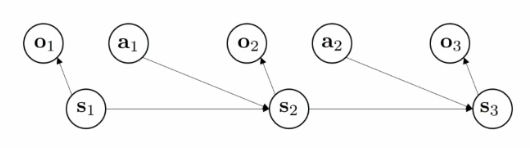
\includegraphics[width=0.6\linewidth]{figures/2020-06-12-185644_530x148_scrot.png}
	\caption{Proceso de decisión de Markov parcialmente observable}
\end{figure}

Como se puede observar, si se conocen los estados las observaciones son independientes.

\section{Definición del problema de RL}%
\label{sec:definición_del_problema_de_rl}

\subsection{El objetivo de RL}%
\label{sub:el_objetivo_de_rl}

El objetivo consiste en encotrar una política que resuelva el problema. En el caso de redes
neuronales, es encontrar los pesos de las neuronas que nos den las acciones correctas dados los
estados.

\[
    p_\theta(s_1,a_1,\ldots,s_T,a_T)=p(s_1) \prod_{t=1}^T \pi_\theta
    (a_t|s_t)p(s_{t+1}|s_t,a_t)
\] 

Probabilidad de pasar por una trayectoria. A partir de ahora $p_\theta(s_1,a_1,\ldots,s_T,a_T)
= p_\theta(\tau)$ 

Se pueden definir objetivos como esperanzas de esta distribución. Se puede escribir un
optimizador para que nos de la solución de esta manera:

\[
    \theta^* =arg\max_\theta E_{\tau \sim p_\theta(\tau)}\left[\sum_t r(s_t, a_t)\right]
\] 

Puede ser que algunos estados no permitan ciertas acciones. Esto realmente no importa ya que se
puede implementar de forma que una acción inválida no produzca ningún cambio.

Una vez se ha escogido una política, se puede considerar que el problema se transforma en una
cadena de markov pero con un espacio de estados distinto.

\begin{figure}[htpb]
	\centering
    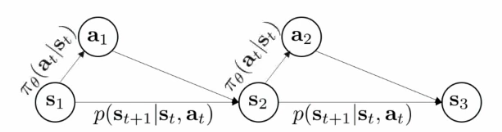
\includegraphics[width=0.8\linewidth]{figures/2020-06-12-190956_502x132_scrot.png}
    \caption{Los nuevos estados están formados por los pares $(s_t, a_t)$}
\end{figure}

Donde las probabilidades de transición pasan a ser:
$p((s_{t+1},a_{t+1})|(s_t,a_t))=p(s_{t+1}|s_t,a_t)\pi_\theta(a_{t+1}|s_{t+1})$

Antes de pasar a plantear el problema con una frontera infinita, se define el marginal
estado-acción.

\begin{align}
    \theta^* &=arg\max_\theta E_{\tau \sim p_\theta(\tau)}\left[\sum_t r(s_t, a_t)\right]\\
             &= arg\max_\theta \sum_{t+1}^{T}E_{(s_t,a_t)\sim p_\theta(s_t,a_t)}[r(s_t,a_t)]
\end{align}

Esto se puede hacer porque la esperanza de un sumatorio es equivalente al sumatorio de la
esperanza. Como el término dentro del sumatorio sólo depende de $(s_t,a_t)$, se puede expresar
como dependiente de $(s_t,a_t)$ en vez de todas las posibles trayectorias.

¿Qué ocurre si $T=\infty$? Dada la condición de que todos los estados sean accesibles desde
todos los otros estados, es decir, que no hayan caminos 'cortados', se demuestra que la
distribución de estados visitados cuando  $T\rightarrow\infty$ se vuelve estacionaria. Se
considerará estacionaria cuando $\mu$ sea el vector propio de $T$ correspondiente al
valor propio 1. Recordar que $\mu$ son los estados de la cadena de markov que están definidos por
$(s_i, a_i)$ y $T$ es la matriz de transición de todos esos estados.

Para el caso del horizonte en el infinito, hay que poner $\frac{1}{T}$ antes del sumatorio a la
hora de calcular $\theta^*$ ya que si no la suma sería infinita. Esto se llama
\textit{undiscounted average return}, y no es muy usado ya que se suelen usar
\textit{discount factors}.

En RL normalmente nos interesa más las esperanzas de las recompensas que las recompensas en sí.
Esto hace que incluso para estados y recompensas discretas la esperanza sea contínua en $\theta$
por lo que los algoritmos de optimización lo tratarán correctamente.

\section{Anatomía de un algoritmo de RL}%
\label{sec:anatomía_de_un_algoritmo_de_rl}

En una forma u otra tienen tres partes:
\begin{itemize}
    \item Generar samples: se consiguen ejecutando la política
    \item Paso de evaluación: hacer una cosa que no cambie la política pero permita evaluarla.
    \item Mejorar la política.
\end{itemize}

\begin{figure}[htpb]
	\centering
	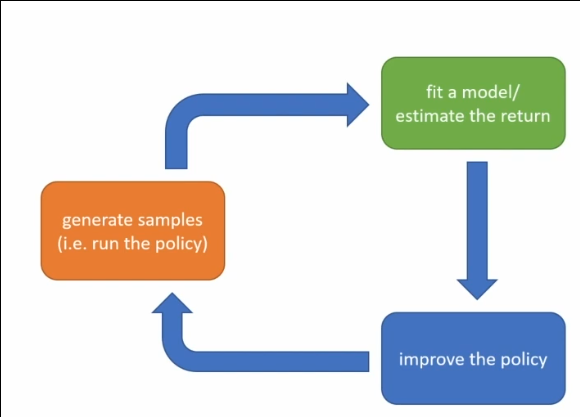
\includegraphics[width=0.8\linewidth]{figures/2020-06-12-193129_580x417_scrot.png}
	\caption{Arquitectura simple de un algoritmo RL}
\end{figure}

\subsection{¿Cómo se gestionan todas las esperanzas?}%
\label{sub:_cómo_se_gestionan_todas_las_esperanzas_}

\begin{align}
    E _ { \tau \sim p _ { \theta } ( \tau ) } \left[ \sum _ { t = 1 } ^ { T } r ( s _ { t } , a _
        { t } ) \right]
\end{align}

Se puede expresar de forma conveniente y recursiva:
\begin{align}
    E _ { s _ { 1 } \sim p ( s _ { 1 } ) } [ E _ { a _ { 1 } \sim \pi ( a _ { 1 } | s _ { 1 } ) } [ r ( s _ { 1 } , a _ { 1 } ) + E _ { s _ { 2 } \sim p ( s _ { 2 } | s _ { 1 } , a _ { 1 } ) } [ E _ { a _ { 2 } \sim \pi ( a _ { 2 } | s _ { 2 } ) } [ r ( s _ { 2 } , a _ { 2 } ) + \ldots | s _ { 2 } ] | s _ { 1 } , a _ { 1 } ] | s _ { 1 } ]
\end{align}
Gracais a la propiedad Markov, la esperanza de $s_3$ dependerá de $(s_2, a_2)$ solamente.

Se define la siguiente función:
\begin{align}
Q ( s _ { 1 } , a _ { 1 } ) = r ( s _ { 1 } , a _ { 1 } ) + E _ { s _ { 2 } \sim p ( s _ { 2 } | s _ { 1 } , a _ { 1 } ) } [ E _ { a _ { 2 } \sim \pi ( a _ { 2 } | s _ { 2 } ) } [ r ( s _ { 2 } , a _ { 2 } ) + \ldots | s _ { 2 } ] | s _ { 1 } , a _ { 1 } ]
\end{align}

La esperanza nos queda así:
\begin{align}
E _ { \tau \sim p _ { \theta } ( \tau ) } [ \sum _ { t = 1 } ^ { T } r ( s _ { t } , a _ { t } ) ] = E _ { s _ { 1 } \sim p ( s _ { 1 } ) } [ E _ { a _ { 1 } \sim \pi ( a _ { 1 } | s _ { 1 } ) } [ Q ( s _ { 1 } , a _ { 1 } ) | s _ { 1 } ] ]
\end{align}

De esta manera es muy fácil modificar $\pi_\theta(a_1|s_1)$ si se conoce $Q(s_1,a_1)$. Por
ejemplo una forma de maximizar la esperanza sería coger la acción que maximice $Q$. Esta
función es la que se conoce como \textit{Q-function}, y se escribe $Q^\pi$ si devuelve la
esperanza que se obtiene con una política $\pi$.

Su contraparte es la función valor, la cual se define como
\begin{align}
V ^ { \pi } ( s _ { t } ) = \sum _ { t ^ { \prime } = t } ^ { T } E _ { \pi _ { \theta } } [ r (
s _ { t ^ { \prime } } , a _ { t ^ { \prime } } ) | s _ { t } ]\\
V ^ { \pi } ( s _ { t } ) = E _ { a _ { t } \sim \pi ( a _ { t } | s _ { t } ) } [ Q ^ { \pi } ( s _ { t } , a _ { t } ) ]
\end{align}

Se discuten las siguientes ideas:
\begin{itemize}
    \item Si se tiene una política $\pi$ y se conoce $Q^\pi$, se puede mejorar la política
        haciendo que esta sea $\pi'(a|s)=1$ si  $arg\max_a Q^\pi(s,a)$. Esta política es tan
        buena o mejor que $\pi$, da igual lo que sea $\pi$.
    \item Se puede usar estas dos funciones para calcular los gradientes que lleven a acciones
        mejores. Si $Q^\pi(s,a) > V^\pi(s)$, entonces  $a$ es mejor que la media, por lo que se
        puede modificar $\pi(a|s)$ para incrementar la probabilidad de $a$.
\end{itemize}

\section{Resumen de los tipos de algoritmos de RL}%
\label{sec:resumen_de_los_tipos_de_algoritmos_de_rl}

\begin{itemize}
    \item \textit{Policy Gradient}
    \item Basados en valor. Calculan los valores óptimos de $V$ o $Q$ y no calculan una
        política.
    \item Es una mezcla de los dos anteriores. Estiman $V$ o $Q$ y optimizan la política.
    \item Basados en modelo: planificación, modelo usado para mejorar la política, u otras
        cosas. Básicamente aprenden $p(s_{t+1} | s_t, a_t)$. Una vez se tiene el modelo, se
        puede hacer planificación (no calcula una política), que consiste en:
        \begin{itemize}
            \item Optimización de trayectorias o control óptimo (principalmente para
                espacios de estado contínuos): esenciaulmente retropropagación
                para optimizar sobre las acciones.
            \item En el caso discreto, se usa por ejemplo \textit{Monte Carlo Tree Search}.
        \end{itemize}
        o se puede retropropagar gradientes en la política, o por último usar el modelo para
        aprender una función de valor mediante programación dinámica.
\end{itemize}

\subsection{¿Por qué hay tantos métodos distintos?}%
\label{sub:_por_qué_hay_tantos_métodos_distintos_}

Porque no se conoce cuál es la mejor forma de resolver el problema. Según el problema, puede ser
interesante que haya un alto \textit{sampling efficiency}, para otros, se busca una mayor
estabilidad o facilidad de uso. También pueden hacerse ciertas asunciones: estocástico o
determinista, contínuo o discreto, episódico o infinito.

\textit{Sampling efficiency} hace referencia a cuantas muestras hacen falta para aprender una
buena política. Es muy importante por ejemplo en casos en los que no se pueda aprender en
simulación.

\begin{itemize}
    \item \textit{Off-policy}: el modelo es capaz de mejorar la política sin generar nuevas
        muestras de la política actual.
    \item \textit{On-policy}: cada vez que se cambie la política, por muy poco que sea, se
        necesitan crear nuevas muestras a partir de dicha política.
\end{itemize}

\begin{figure}[htpb]
	\centering
	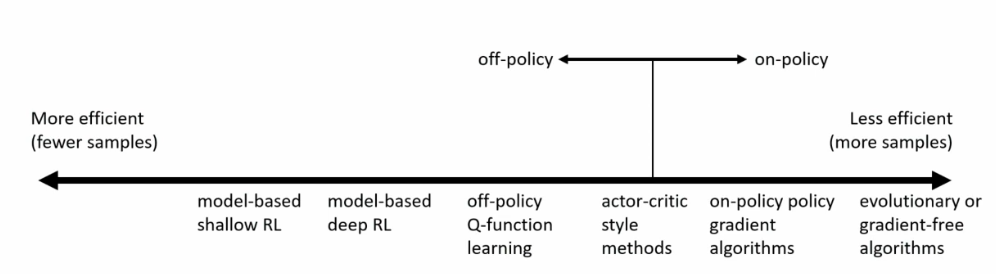
\includegraphics[width=0.8\linewidth]{figures/2020-06-12-202343_996x274_scrot.png}
	\caption{Eficiencia de varios algoritmos de RL}
\end{figure}

\textit{Sample efficiency} suele ir invertido con la eficiencia en la práctica. Si se
tiene un simulador que sea casi instantáneo, casi siempre un algoritmo genético aprenderá
mucho más rápido (en tiempo real). Esto es así porque son mucho más paralelizables y
menos costosos computacionalmente.

Hay otras consideraciones, como que los modelos que están más a la izquierda suelen hacer
asunciones más fuertes que los de la derecha. Por ejemplo \textit{Q-learning} requiere
de observabilidad completa del estado markoviano.

También se tienen que hacer las siguientes preguntas:
\begin{itemize}
    \item ¿El modelo converge?
    \item ¿Si es así, a qué?
    \item ¿Converge siempre?
\end{itemize}

Estas preguntas tienen sentido por motivos como los siguientes:
\begin{itemize}
    \item \textit{Q-learning} no es descenso por gradiente, es una iteración de punto fijo.
    \item Los algoritmos basados en modelo no optimizan la esperanza de la recompensa.
    \item \textit{Policy Gradient} si que es descenso por gradiente, pero es el más ineficiente.
\end{itemize}
